\section{Background and Motivation}
\vspace{-.5em}
Failures such as process crash, kernel panics, power outages are commonplace in today's systems, and
very likely introduce fatal effects to applications such as data inconsistency or loss. 
To be resilient to failures, mission-critical applications often store their data in transactional databases, which rely on write-ahead logging to make updates persistent to non-volatile storage upon transaction commits and recover system state from failures when failures reboot. As users favor real-time responses and highly available services, the performance of runtime logging and offline recovery is crucial. 

However, a recent study concluded that logging is one of the bottlenecks in databases 
running on multi-core machines by showing that a significant amount of CPU cycles corresponds 
to log contentions~\cite{Wang2014DistLog}. The root cause of the slowdown is that the widely used logging and 
recovery algorithms such as ARIES~\cite{Mohan1992ARIES} maintain a single log and many concurrent threads contend for the log head. Similarly, recovering performs poorly as it needs to sequentially scan the whole log and does not explore massive parallelism enabled by current hardware. This result points out there exists a gap between the original design principles of database logging and the ever increasing CPU density and capacity. 

To close the gap, some researchers proposed to keep a set of distributed logs rather than a centralized log so that the log contentions will be reduced~\cite{Wang2014DistLog}. However, the major challenge of doing so is to maintain consistency between log entries across multiple log files, which hinders the recovery performance due to the following reasons. First, dependencies between log entries belonging to different transactions lead to cross-log synchronizations when recovering state from failures, as their relative orders matter~\cite{Johnson2012Scale}. Second, the ordering constraints between entries imposed at the logging time is stronger than those established when their corresponding transactions were executing. Third, there exist many false dependencies introduced by logging changes to pages, as two transactions modifying different parts of a shared page will be still flagged as conflicting. 

\if 0
Generally, systems leverage single Log to log and recover for simple, this is why the logging and revovery are so slow. First, the multiple threads will contend to write to a single Log, second, a sequential scan will be performed over the corresponding log by only one thread. Both of them will cause worse scalability as the number of threads grows in a single node with multi-core.

A straightforward approach to speed up the logging and recovery is distributing the Log, for example, one Log file per processor. But the distributed Log is still tardy because of too many cross-log dependencies.

In this paper, we propose a new version of distributed Log by leveraging a few techniques, which will support parallelism well in single node with multi-core.
% Modern distributed file systems, such as GFS\cite{ghemawat2003google}, HDFS\cite{shvachko2010hadoop}, Ceph\cite{weil2006ceph}, which consist of three components, metadata servers(MDS), object-based storage devices(OSD) and clients as Fig.~\ref{fig:architecture} shows. Clients perform metadata operations(\emph{open, stat}) directly with MDS and file I/O directly with data server. This architecture decouples metadata I/O from data IO and increases overall scalability. For example, client requests data with pathname /var/log/client.log. By multiple interactions to MDS, client lookups the directory of \texttt{root}, \texttt{var} and \texttt{log} to locate the inode of \texttt{client.log} and checks the permission. Once client obtain the inode, it must get the capability to access to data. Then, client will request a lease on this file to MDS. Finnaly, client interact with OSD to operator file I/O. Due to the iterative lookup and checking permission operations, the IOs between clients and MDS are more than OSD. Because overall 50\% of IOs are to metadata\cite{roselli2000comparison}, metadata performance is crucial.

% \begin{figure}[htbp]
%   \centering
%   % Requires \usepackage{graphicx}
%   %\vspace{-5pt}
%   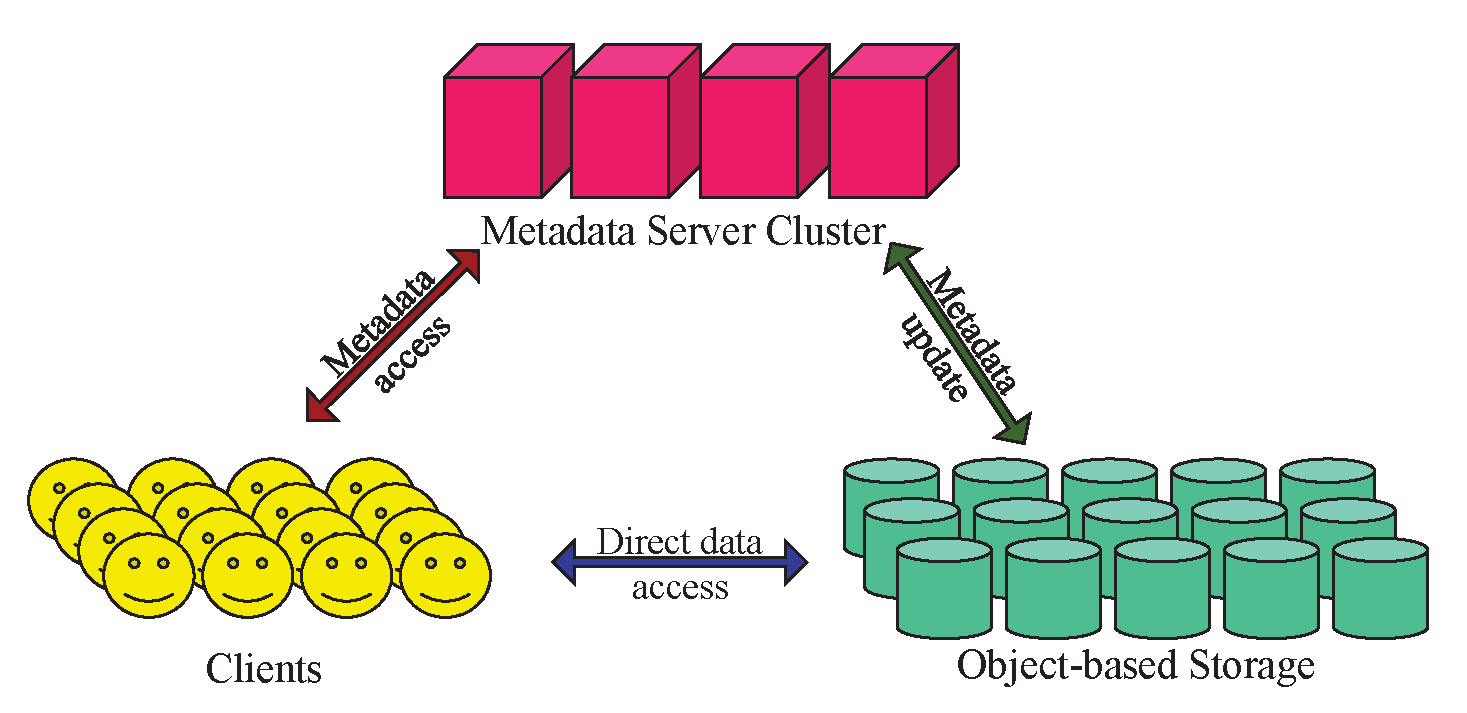
\includegraphics[width=1\linewidth]{architecture.eps}\\
%   %\vspace{-10pt}
%   \caption{Architecture of distributed file systems.}\label{fig:architecture}
%    %\vspace{-10pt}
% \end{figure}
\begin{figure}[htbp]
  \centering
  % Requires \usepackage{graphicx}
  %\vspace{-5pt}
  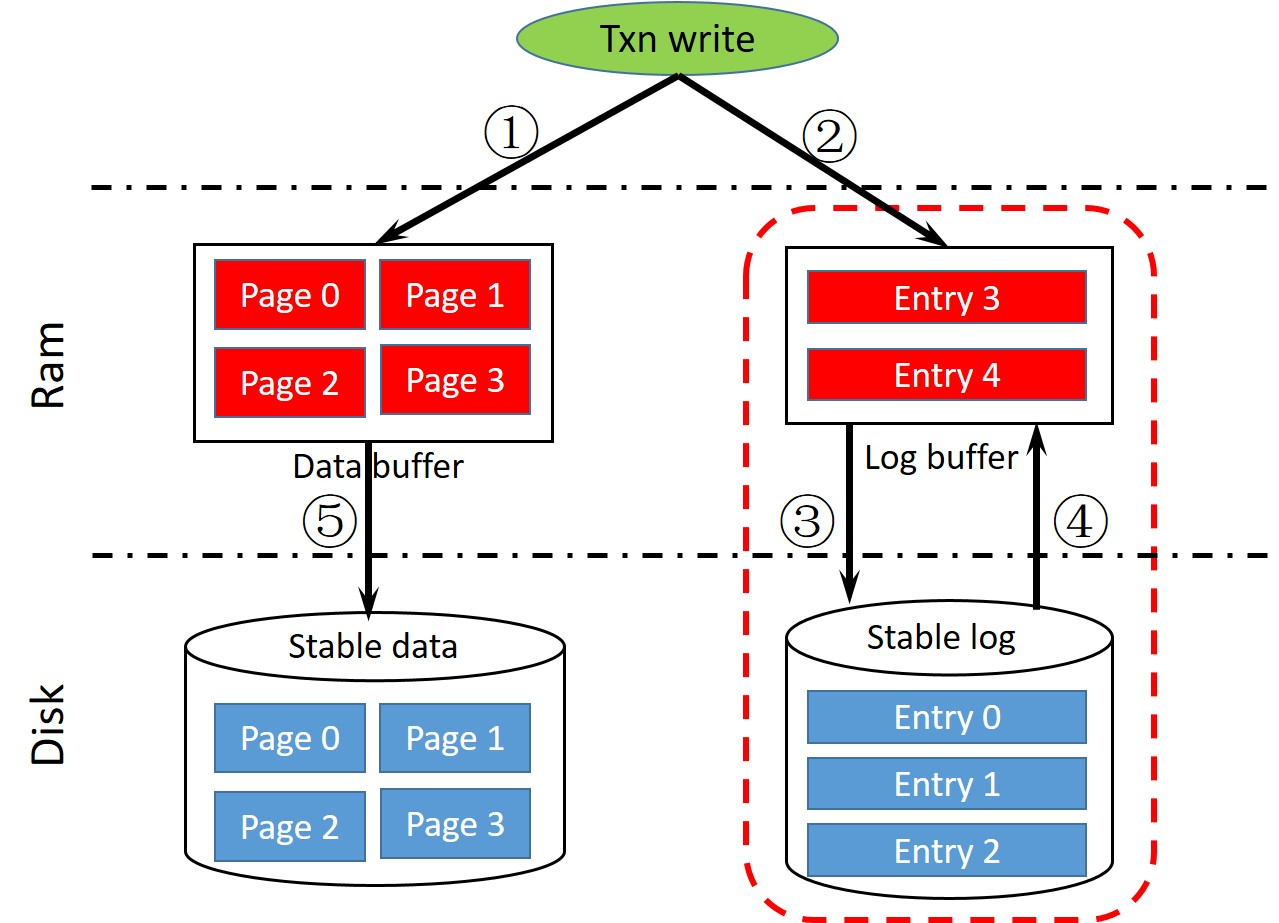
\includegraphics[width=1\linewidth]{architecture.jpg}\\
  %\vspace{-10pt}
  \caption{Architecture and process flow of write-ahead logging.}\label{fig:architecture}
   %\vspace{-10pt}
\end{figure}

\fi
% In this paper, we propose a correlations-based metadata prefetching to reduce IO traffic to MDS, to scale distributed file systems, to increase client cache hit ratio with high accuracy and low false positive. How to define the correlations among files and how to update correlations in real time become a challenge.
